\documentclass[10pt,letterpaper]{article}
\usepackage[top=0.85in,left=2.75in,footskip=0.75in,marginparwidth=2in]{geometry}

% use Unicode characters - try changing the option if you run into troubles with special characters (e.g. umlauts)
\usepackage[utf8]{inputenc}

% clean citations
\usepackage{cite}

% hyperref makes references clicky. use \url{www.example.com} or \href{www.example.com}{description} to add a clicky url
\usepackage{nameref,hyperref}

\usepackage{amsmath}

% line numbers
\usepackage[right]{lineno}
% improves typesetting in LaTeX
\usepackage{microtype}
\DisableLigatures[f]{encoding = *, family = * }

% text layout - change as needed
\raggedright
\setlength{\parindent}{0.5cm}
\textwidth 5.25in 
\textheight 8.75in

% Remove % for double line spacing
\usepackage{setspace} 
\doublespacing

% use adjustwidth environment to exceed text width (see examples in text)
\usepackage{changepage}

% adjust caption style
\usepackage[aboveskip=1pt,labelfont=bf,labelsep=period,singlelinecheck=off]{caption}

% remove brackets from references
\makeatletter
\renewcommand{\@biblabel}[1]{\quad#1.}
\makeatother

% headrule, footrule and page numbers
\usepackage{lastpage,fancyhdr,graphicx}
\usepackage{epstopdf}
\pagestyle{myheadings}
\pagestyle{fancy}
\fancyhf{}
\rfoot{\thepage/\pageref{LastPage}}
\renewcommand{\footrule}{\hrule height 2pt \vspace{2mm}}
\fancyheadoffset[L]{2.25in}
\fancyfootoffset[L]{2.25in}

\lfoot{\today}

% use \textcolor{color}{text} for colored text (e.g. highlight to-do areas)
\usepackage{xcolor}

% strike
\usepackage{soul}

\newcommand{\blu}{\textcolor{blue}}

% define custom colors (this one is for figure captions)
\definecolor{Gray}{gray}{.25}

% this is required to include graphics
\usepackage{graphicx}

% use if you want to put caption to the side of the figure - see example in text
\usepackage{sidecap}

\usepackage{epigraph} 
% \usepackage[options]{nohyperref}
\usepackage{soul}

% math stuff
\usepackage{amssymb}
\usepackage{amsfonts}
\usepackage{blkarray}
% use for have text wrap around figures
\usepackage{wrapfig}
\usepackage[pscoord]{eso-pic}
\usepackage[fulladjust]{marginnote}
\reversemarginpar

% abbriviations
\newcommand{\ecoli}{\emph{E. coli} OP50}
\newcommand{\novo}{\emph{Novosphingobium} sp. L76}
\newcommand{\ppac}{\emph{P. pacificus}}

% document begins here
\begin{document}
\vspace*{0.35in}

% title goes here:
\begin{flushleft}
{\Large
\textbf\newline{Spatial and temporal heterogeneity alter the cost of plasticity in \emph{Pristionchus pacificus}}}
\newline
% \vspace*{0.1in}


% % authors go here:
% \vspace*{0.1in}
Ata Kalirad\textsuperscript{1},
Ralf J. Sommer\textsuperscript{1,*}
\\
\bigskip
\bf{1} Department for Integrative Evolutionary Biology, Max Planck Institute for Biology T{\"u}bingen, 72076 T{\"u}bingen, Germany
\\

\bigskip
* ralf.sommer@tuebingen.mpg.de

\bigskip
ORCID: 0000-0002-9500-3903 (AK) \\
ORCID: 0000-0003-1503-7749 (RJS)

\end{flushleft}

% \setcounter{figure}{1}

\section*{Abstract}

Phenotypic plasticity, the ability of a single genotype to produce distinct phenotypes under different environmental conditions, has become a leading concept in ecology and evolutionary biology, with the most extreme examples being the formation of alternative phenotypes (polyphenisms). However, several aspects associated with phenotypic plasticity remain controversial, such as the existence of associated costs. While already predicted by some of the pioneers of plasticity research, i.e. Schmalhausen and Bradshaw, experimental and theoretical approaches have provided limited support for the costs of plasticity. In experimental studies, one common restriction is the measurement of all relevant parameters over long time periods. Similarly, theoretical studies rarely use modelling approaches that incorporate specific experimentally-derived fitness parameters. Therefore, the existence of the costs of plasticity remains disputed. Here, we provide an integrative approach to understand the cost of adaptive plasticity and its ecological ramifications, by combining laboratory data from the nematode plasticity model system \emph{Pristionchus pacificus} with a stage-structured population model. Taking advantage of measurements of two isogenic strains grown on two distinct diets, we illustrate how spatial and temporal heterogeneity with regards to the distribution of resources on a metapopulation can alter the outcome of the competition and alleviate the realized cost of plasticity.

\hspace{5cm}

\noindent
\textbf{Keywords:} Phenotypic plasticity, cannibalism, cost of plasticity, metapopulation models

\noindent
\textbf{Short title:} Spatial and temporal heterogeneity alters the cost of plasticity 

\section*{Author Summary}

The ability of living organisms to express different phenotypes without genetic change (phenotypic plasticity) has fascinated biologists, probably since the establishment of biology as a branch of science. Despite its ubiquity in nature, many aspects of phenotypic plasticity remain unresolved. For instance, it has been suggested that a biological system equipped with phenotypic plasticity would necessarily have to pay a cost in fitness compared to a non-plastic counterpart. In this manuscript, we utilize the laboratory data on the nematode plasticity model system \emph{Pristionchus pacificus} to simulate how the cost of plasticity would manifest itself in a competition between a plastic and a non-plastic organism. This nematode exhibits predatory mouth under certain environmental conditions, including diet. We show how variation in the distribution of resources in space and time can greatly affect the outcome of competition. Our work illustrates the complexity of predicting the ecological consequences of phenotypic plasticity in a changing world. 
% % now start line numbers
\linenumbers

% % the * after section prevents numbering

% \epigraph{Thus there is only too often the problem of formulating the problem—and the problem whether this was really the problem to be formulated.}{\textit{Karl Popper\cite{Popper1992}}}


\section*{INTRODUCTION}

% \subsection*{The cost of (adaptive) plasticity and its discontents}

The expression of alternative phenotypes by a single genotype in different environments, i.e., phenotypic plasticity or polyphenism, remains a topic of great interest and discussion in both ecology and evolution \cite{Schmalhausen1949, Waddington1957, Eberhard2003, Sommer2020a}. A plastic organism capable of assuming the form and function fitted to multiple environments could have a considerable advantage in competition against genetically hard-wired competitors. However, intuitively, such adaptive plasticity, given the hypothetical machinery behind it, should  incur a cost. This possible cost did not escape the pioneers in the study of plasticity; for example, Bradshaw argued that a case of adaptive plasticity could be selected against if the plastic trait were too costly \cite{Bradshaw1965}. This hypothetical cost of adaptive plasticity, has ever since been analyzed, elaborated upon, and reviewed in the literature (e.g., see \cite{Newman1992, DeWitt1998, Murren2015, Forsman2015, Agrawal2020}). 

\hspace{5cm}

It should be noted that, curiously, the term ``cost of plasticity'' is sometimes used in reference to the aforementioned hypothesis, for example see \cite{Callahan2008, Agrawal2020}, even though the purported fitness trade-off can only be attributed to plasticity when it is adaptive. While this rather minute ambiguity reflects the extensive interchangeable usage of ``plasticity'' and ``adaptive plasticity'' in the literature, it should be avoided, since, as pointed out by Bradshaw, ``the concept of plasticity does not also have any implications concerning the adaptive value of the changes occurring [...]" \cite{Bradshaw1965}.  

\hspace{5cm}

There have been many attempts to measure the cost of adaptive plasticity in nature (e.g., \cite{Krebs1997, Smekens2001, STEINER2008}). The general design of such studies involves finding a plastic trait that can be plausibly characterized as adaptive with regards to a given environmental condition, and measuring a component of fitness, e.g., fecundity, size, etc., across two or more conditions, one being the condition to which the plastic response is adapted. While such studies should, in principle, demonstrate the cost of plasticity, they have provided mixed evidence; a meta-analysis of 27 studies of the cost of adaptive plasticity concluded that the costs measured in these studies are quite infinitesimal, if present at all \cite{BUSKIRK2009}. Surprisingly, while \emph{Daphnia} is sometimes used as a visual aide to illustrate the cost of adaptive plasticity (e.g., \cite{Pfennig2021}), the induction of the defensive spine in \emph{Daphnia pulex}, in response to a predator (\emph{Chaoborus americanus}), was shown to have negligible cost in spite of a forgiving statistical approach\cite{Scheiner1998}. 

% The theoretical ramifications of the cost of adaptive plasticity was explored by Van Tienderen \cite{Tienderen1991}. In this two-patch model, Van Tienderen explored effect of the cost of being a ``jack-of-all trades'' in comparison to a specialist genotype, using a Gaussian cost function. This 

\hspace{5cm}

On the theoretical front, attempts have been made to provide concrete theoretical predictions with regards to the effect of the cost of adaptive plasticity. In one of the earliest examples, Van Tienderen \cite{Tienderen1991} analyzed the cost of adaptive plasticity in an arbitrary quantitative trait with a Gaussian cost function. While his model predicts scenarios in which the plastic genotype could coexist with the specialist one, the results are dependent on the initial condition and the selection regime, among others. In a more recent study, Doret \emph{et al.} \cite{Doret2020} use a modified Gillespie algorithm to simulate a model of gene network to investigate the cost of adaptive plasticity. They distinguished between two possible mechanisms for the plastic response to the environmental change: environmental signal and performance signal, the latter being an endogenous signal that indicates how well the organism is functioning in a given environment. They concluded that being plastic is only costly when the developmental system relies on the environmental signal. This result is intriguing, but, since Doret \emph{et al.} measured cost via the robustness of the development, any attempt to relate their results to the experimental measurements of the cost of adaptive plasticity, in which a component of fitness is measured, should proceed with a modicum of caution. 

\hspace{5cm}

The experimental and theoretical approaches mentioned above, and many other similar works, have contributed to an extensive body of work on adaptive plasticity. However, given the paucity of support for costs of plasticity in the wild and the nature of the theoretical works on this topic, the existence of such costs remains a matter of debate. One could shed more light on this phenomenon by melding relevant experimental data on the differential response to environmental fluctuations with a modelling approach. Specifically, modelling of the population dynamics to extrapolate from experimental snapshots observed in the wild or the laboratory, can provide computational predictions of the ecological consequences of adaptive plastic responses and their purported costs. Here, we provide an example of this integrative approach to understand the cost of adaptive plasticity and its ecological ramifications, by combining laboratory data from the nematode \emph{Pristionchus pacificus} with a modified stage-structured metapopulation model. 

\hspace{5cm}

\ppac{} is a well-established model system to study phenotypic plasticity \cite{Sommer2013a}. The mouth form of this hermaphroditic nematode can assume two alternative states: a wide eurystomatous (predatory) form with two teeth, which enables the nematode to prey upon other nematodes, and a narrow bacterivorous stenostomatous (non-predatory) form with a single tooth (Figure \ref{fig:fig1}a). It is important to note that only the eurystomatous form is a predator of other nematodes and only adult worms can kill. \ppac{} and its relatives are soil nematodes that are most reliably found in association with scarab beetles \cite{Herrmann2007a, KANZAKI2021}. These nematodes stay in the arrested dauer larval stage (an alternative larval stage) as long as the adult beetle is alive and flourish on the beetle cadaver in the soil once the beetle has died \cite{Meyer2017a, Renahan2021aa} (Figure \ref{fig:fig1}b). Mouth-form plasticity and intraguild predation are important life history traits in the short-lived and competitive ecosystem of the decaying beetle, where the expression of the predatory mouth form can seemingly fluctuate over time in response to competition \cite{Renahan2021aa, Renahan2022a}. The state of the mouth form can be influenced by a variety of stimuli, including temperature, culture methods, pheromones, and bacterial diet \cite{Lenuzzi2021, Werner2017, Werner2018a, Akduman2020a}. In addition to change in mouth form due to environmental cues, different wild isolates of \ppac{} exhibit a range of mouth-form ratios under laboratory condition \cite{Ragsdale2013}. Given that the molecular machinery regulating mouth-form plasticity in \ppac{} has been identified \cite{Kieninger2016, Sieriebriennikov2018, Bui2018, Namdeo2018, Sieriebriennikov2020}, this study system has the prospect of merging experimental and theoretical approaches of plasticity research and associated boundary conditions, such as the costs of adaptive plasticity.   

\hspace{5cm}

Previously, we demonstrated the cost of plasticity and the cost of phenotype in \ppac{} by measuring the fecundity - as a proxy for fitness - of two isogenic strains of this nematode across two alternative diets \cite{Dardiry2023}. On \novo{} (the inducing diet), the probability of developing the predatory mouth form of the plastic strain increases drastically from a low probability of expressing this phenotype on \ecoli{} (the non-inducing diet). The adults of the non-plastic strain express the predatory phenotype across both conditions. Our experimental measurements of fecundity revealed a significant cost of plasticity in the plastic strain, as well as cost of phenotype in the non-plastic strain (Figure \ref{fig:fig1}c). We incorporated the fecundity and experimental data in a stage-structured model to further illustrate the effects of the costs of plasticity and phenotype on the population dynamics.

\hspace{5cm}

In this study, we address some of the limitations of our previous computational attempts by investigating the interplay between costs of phenotype and plasticity in \ppac{} strains in a stage-structured metapopulation model consisting of an $m\times m$ lattice. Using experimentally-estimated parameters for developmental speed, fecundity, and mouth-form plasticity, we simulate the population dynamics of the plastic and the non-plastic strains on a metapopulation. We illustrate how environmental heterogeneity in space and time can alleviate the inferred cost of plasticity. This study highlights the complexity of predicting the cost of plasticity and its ecological consequences in variable conditions. 

\section*{MATERIALS AND METHODS}

To simulate the population dynamics of the interaction between the plastic and the non-plastic strains of \ppac{}, we use a modified version of a stage-structured matrix population model used in \cite{Dardiry2023}. In this model, we envision the life cycle of \ppac{} as an absorbing finite-state Markov chain \cite{Keyfitz2005, Caswell2019} (Fig. \ref{fig:fig1}b). The life cycle consists of egg (E), juvenile (J), dauer larvae (d), young adult (YA), reproducing adult (RA), and old adult stages (OA). The dynamics of the population of strain $i$ is determined by its transition matrix $\mathbf{U}_{R,i}$ and its fecundity matrix $\mathbf{F}_{R,i}$, both of which are resource and strain dependent. For strain $i$, the transition matrix is

\begin{adjustwidth}{-2in}{0in}
\[ \mathbf{U_{R,i}}= \begin{blockarray}{cccccccc}
\mathrm{E} & \mathrm{J} & \mathrm{d} & \mathrm{YA} & \mathrm{RA}_1 & \hdots & \mathrm{RA}_5& \mathrm{OA} \\
\begin{block}{(cccccccc)}
\sigma_1 (1- \gamma_{21}) & 0 & 0 & 0 & 0 & \hdots & 0 & 0\\
\sigma_1 \gamma_{21} & \sigma_2 (1- \gamma_{32}) (1- \gamma_{42}) & 0 & 0 & 0 & \hdots & 0 & 0\\
0 & \sigma_2 \gamma_{32} & \sigma_3(1 - \gamma_{43}) & 0 & 0 & \hdots & 0 & 0\\
0 & \sigma_2\gamma_{42} & \sigma_3\gamma_{43} & \sigma_4(1 - \gamma_{54})  & 0 & \hdots & 0 & 0\\
0 & 0 & 0 & \sigma_4 \gamma_{54} & \sigma_5 (1 - \gamma_{65}) & \hdots & 0 & 0\\
\vdots & \vdots & \vdots & \vdots & \vdots & \vdots & \vdots & \vdots \\
0 & 0 & 0 & 0 & 0 & \hdots & \sigma_9 (1 - \gamma_{109})  & 0\\
0 & 0 & 0 & 0 & 0 & \hdots & \sigma_9 \gamma_{109}  & \sigma_{10}\\  
\end{block} 
\end{blockarray}  \quad . \] %
\end{adjustwidth}

The transition from juvenile to dauer larvea only occurs when resource reaches an arbitrary minimum. When resource is available, dauer larvae transit into the young adult stage. The YA to RA$_i$ transition rate is strain and resource dependent and reflects the change in the developmental speeds of the plastic and the non-plastic strains on \ecoli{} and \novo{}\cite{Dardiry2023}. The survival probabilities of all stages, except for the dauer stage, depends on resource availability as well, while $\sigma_{\mathrm{dauer}}=1$ to reflect the observation that \ppac{} can survive as dauer larvae for up to 50 weeks under laboratory conditions \cite{Mayer2011aa} (for detailed effect of amount and type of resource on transition and survival probabilities, see Fig.\ref{fig:figs1}).

\hspace{5cm}

The entries in $\mathbf{F}_{R,i}$ are based on the average number of eggs laid by the non-plastic and the plastic strains on \emph{E. coli} and \novo{} \cite{Dardiry2023}. The mean number of eggs laid are used to construct the fecundity matrix:

\begin{equation}
\mathbf{F_{R,i}} = 
\begin{pmatrix}
0 & \cdots & f_1(R,i) & \cdots & f_5(R,i) & 0 \\
0 & \cdots & \cdots & \cdots & \cdots & 0 \\
\vdots & \cdots & \cdots & \cdots & \cdots & \vdots \\
0 & \cdots & \cdots & \cdots & \cdots & 0 \\
\end{pmatrix} \quad ,
\end{equation}

where $f_j(R,i)$ is the mean number of eggs laid by the breeding adult of day $j$ from strain $i$ on resource type $R$ multiplied by the probability of transition from the reproducing adult of day $j$ to the reproducing adult of day $j + 1$ or the old adult (Table \ref{table:fec}).

\hspace{5cm}

Resource consumption is modeled in a linear fashion. Given $\mathcal{R}_t$, the amount of available resource at the next step will be:

\begin{equation}
    \mathcal{R}_{t + 1}  = \mathcal{R}_{t} - \rho n_c \quad ,  \mathcal{R}_{t + 1} \geqslant 0 \quad ,
\label{eq:food}
\end{equation}

where $\rho$ is the consumption rate and $n_c$ is number of consumers in the population, which excludes eggs and dauer larvae. 

\hspace{5cm}

The population is represented by a vector

\begin{equation}
\mathbf{n} = 
\begin{pmatrix}
n_{i1}  \\
\vdots  \\
n_{i10}  \\
\rule{0.05\textwidth}{0.5pt} \\
n_{j1}  \\
\vdots  \\
n_{j10}   \\
\end{pmatrix} \quad ,
\end{equation}

where $n_{l m}$ represent the number of individuals that belong to stage $m$ of the strain $l$. The composition of the population in the next step, without taking into account predation and dispersal, will be
\begin{equation}
    \mathbf{n} (t+1) = \mathbb{A}(t)  \mathbf{n} (t) \quad ,
\label{eq:projection}
\end{equation}

where

\begin{equation}
\mathbb{A}(t) = 
\begin{pmatrix}
\mathbf{U}(i,t) + \mathbf{F}(i,t) &  \\
& \mathbf{U}(j,t) + \mathbf{F}(j,t)\\
\end{pmatrix} \quad .
\end{equation}

\hspace{5cm}

The effect of predation of strain $j$ on strain $i$ at each step is included as a simple type I predation:

\begin{equation}
    \phi_{i}(t) = \alpha \lambda_j(t) n_{jA}(t) n_{im}(t) \quad , \phi_{i}(t) \leqslant  n_{im}(t)  \quad ,
\label{eq:pred}
\end{equation}

where $\alpha$ is the predation rate, $\lambda_j(t)$ is the expected proportion of predatory adults of strain $j$ at time $t$, $n_{jA}(t)$ is the number of adults (reproducing adult and old adult stages) of strain $j$ at time $t$, and $n_{im}(t)$ is the number of individuals of strain $i$ at the time $t$ that belong to the potential pray stages (juvenile or dauer larvae, $m=2,3$). For the non-plastic strain, $\lambda=1$ regardless of the bacterial diet, while for the plastic strain, $\lambda=0.11$ on \ecoli{} and $\lambda=0.83$ on \novo{}. 

%The total number of adults of strain $j$, $n_{jA}(t)$, includes all five reproducing adult stages and the old adult stage.

\hspace{5cm}

In nature, upon the depletion of bacteria on the beetle carcass, \ppac{} dauer larvae are generated and rapidly disperse in the surrounding soil \cite{Renahan2021aa}. The dispersion of dauer larvae across the metapopulation is modeled as a simple diffusion model \cite{Downey2018}, where the diffusion of dauer larvae from subpopulation $S_{ij}$ is simulated by comparing the frequencies of dauer larvae, $f(\mathrm{dauer})$, in this subpopulation to its neighbors in a von Neumann neighborhood and applying a diffusion kernel to this neighborhood. The kernel approximates $\nabla^2 f(\mathrm{dauer})$. The rate of dispersal is determined by the diffusion rate $r$.

\hspace{5cm}

The expected composition of metapopulation at time $t+1$ is calculated in three steps:

\begin{enumerate}
    \item For each of the $m^2$ subpopulations in the metapopulation, the  expected population composition without predation at $t+1$ is calculated using Eq. \ref{eq:projection}.

    \item Calculating the effect of predation on the number juvenile and dauer larvae in each subpopulation using Eq. \ref{eq:pred}.

    \item The dauer larvae disperse across the metapopulation from any given subpopulation to its neighbors according to $r \nabla^2 f(\mathrm{dauer})$. 
\end{enumerate}


% By including predation and dispersion, the expected composition of a population at time $t+1$ would be

% \begin{equation}
%     \mathbf{n}(t+1) = \mathbb{A}(t)\mathbf{n}(t) - 
%     \begin{pmatrix}
% 0  \\
% \phi_{i2}(t)\\
% \phi_{i3}(t)\\
% 0 \\
% \vdots  \\
% \rule{0.05\textwidth}{0.5pt} \\
% 0  \\
% \phi_{j2}(t)\\
% \phi_{j3}(t)\\
% 0 \\
% \vdots  \\
% \end{pmatrix} - 
%     \begin{pmatrix}
% 0  \\
% 0 \\
% \omega_{i3}(t)\\
% 0 \\
% \vdots  \\
% \rule{0.05\textwidth}{0.5pt} \\
% % \hline
% \vdots \\
% \omega_{j3}(t)\\
% 0 \\
% \vdots  \\
% \end{pmatrix}
% \quad ,
% \end{equation}

% where $\phi_{lm}(t)$ is the effect predation of stage $m$ of strain $l$ and $\omega_{l3}$ is the effect of the dispersion on the number of dauer larvae of strain $l$.

\hspace{5cm}

\begin{table}[h!]
\centering
\begin{tabular}{|p{2cm}|p{1cm}|p{1cm}|p{1cm}|p{1cm}|p{1cm}|}
 \hline
& \multicolumn{2}{c}{\ecoli{}} & \multicolumn{2}{|c|}{\novo{}}\\
    \cline{1-2}
 \hline
Adult stage & $m_{P}$ & $m_{NP}$ & $m_{P}$ & $m_{NP}$ \\
 \hline
 RA$_1$ & 22.65 & 19.8 & 11.66 & 16.88 \\
 RA$_2$ & 68.45 & 60.3 & 62.53 & 80.77 \\
  RA$_3$ & 57.05 & 43.02 & 47.13 & 77.7 \\
   RA$_4$ & 33.4 & 19.9 & 13.94 & 16.28 \\
    RA$_5$ & 4.97 & 6.6 & 0.72 & 1.4 \\
    \hline 
    $R_0$ & 186.52 & 149.62 & 135.98 & 193.03 \\
 \hline
\end{tabular}
\caption{The fecundity ($m$) of the five reproducing adult stages in our model for the plastic (P) and the non-plastic (NP) strains on two different bacterial diets based on the laboratory measurements. $R_0$ is the rate of increase per generation, given by the leading eigenvalue of $\mathbf{F} \mathbf{N}$, where $\mathbf{F}$ is the fecundity matrix and $\mathbf{N}$ is the fundamental matrix of a given transition matrix \cite{Cushing1994}.}
\label{table:fec}
\end{table}


\section*{Data and code availability}

The software used to run all simulation was written in Python 3.10.4 with NumPy 1.21.5 \cite{har20i}. The diffusion was simulated using \texttt{correlate2d} in SciPy 1.7.1 \cite{2020SciPy-NMeth}. The code and the data are available at the GitHub repository associated with this manuscript (\url{https://github.com/Kalirad/MetaPopProjection}).

% \hspace{5cm}

% The software used to run all simulations was written in Python 3.10 with NumPy\cite{Harris2020} version 1.22.3. All code and data are available at \url{https://github.com/Kalirad/https://github.com/Kalirad/MetaPopProjection}.

\section*{RESULTS}

We used experimentally-derived life history parameters of two wild isolates of \ppac{} to study the cost of plasticity \cite{Dardiry2023}. Before simulating competition between the plastic and the non-plastic strains, we simulated the population dynamics of each strain individually with unlimited food source (Fig.\ref{fig:fig1}d). In isolation, the dynamics of the plastic and the non-plastic strains is consistent with both the cost of phenotype, the lower growth rate of the non-plastic strain in the non-inducing environment (\ecoli{}) relative to the plastic strain, and the cost of plasticity, the lower relative growth rate of the plastic strain on the inducing environment (Fig. \ref{fig:fig1}c-d). What complicates the issue of cost in this context is the fact that the induced phenotype in the plastic strain is the increase in the proportion of the predatory mouth form from $0.11$ on \ecoli{} to $0.83$ on \novo{}(Fig. \ref{fig:fig1}c). Specifically, the predatory nature of the plastic phenotype raises an interesting question: if we include the induced phenotype, does the predation of juvenile and dauer larval stages of the non-plastic strain by the plastic strain offset the cost of plasticity? We address this question using a stage-structured population model, which will subsequently be extended to a metapopulation model.

\hspace{5cm}

Next, we simulated the dynamics of the two strains in a well-mixed population, with and without predation (Fig. \ref{fig:fig2}a). In the absence of predation, the plastic strain reaches a higher abundance in all stages compared to the non-plastic strain on \ecoli{}, given its higher relative growth rate, while it fares worse on \novo{}. If we were to include predation, the non-plastic strain always competitively excludes the plastic strain regardless of the diet. Thus, the magnitude of the induced phenotype in the plastic strain is not enough to offset the lower relative growth rate of this strain on \novo{} (Fig. \ref{fig:fig2}a). However, the will-mixed condition is an extreme case, and in nature one would expect heterogeneity both in space and time. To capture these aspects, we constructed a metapopulation model (Fig. \ref{fig:fig2}b). Here, the strains can develop in each subpopulation, and once the food is depleted, dauer larvae are produced and diffuse across the metapopulation (Fig. \ref{fig:fig2}c). In a simple spatial arrangement, the higher growth rate of the plastic strain on \ecoli{}, and the cost of phenotype that burdens the non-plastic strain on this diet, results in the plastic strain dominating a $10 \times 10$ metapopulation, both in terms of the abundance of reproducing adults and dauer larvae (Fig. \ref{fig:fig2}d, \nameref{S1_Video}). In contrast, on the \novo{} diet, the non-plastic strain remains dominant (Fig. \ref{fig:fig2}d). Together, these simulations highlight the effect of introducing spatial heterogeneity on the competition between the strains, resulting in opposite competitive outcomes. 

\hspace{5cm}

In nature one would expect a heterogeneous distribution of resource, both with regards to amount and type. To explore the effect of non-homogeneous distribution of resource type in the environment, we simulated the population dynamics over metapopulations with two arbitrary resource distribution patterns: in each pattern, the metapopulation was divided into four quadrants and either \ecoli{} or \novo{} was assigned to each quadrant (Fig.\ref{fig:fig3}a-b). The expectation is that, given the effect of each diet on developmental speed, specifically ($\mathrm{YA} \rightarrow \mathrm{RA}_1$), and fecundity of the two strains, these heterogeneities will influence the realized costs of plasticity and phenotype, such that the competitive outcomes over the metapopulation will be altered. Indeed, this expectation is validated in one of the two arbitrary arrangements. If the plastic strain starts on the non-inducing condition, the non-plastic strain will out-compete the plastic strain in this pattern (Fig. \ref{fig:fig3}a). In contrast, if the plastic strain starts on the inducing condition, its competitive capability increases (Fig. \ref{fig:fig3}b, \nameref{S2_Video}). Furthermore, if we assign resource type to subpopulations at random, different competitive outcomes emerge, some favoring the plastic strain (Fig. \ref{fig:fig3}c and Fig. \ref{fig:figs2}). Thus, heterogeneous distribution of resource also results in opposite outcomes. 

\hspace{5cm}

There are two limitations to the previous exploration of the effect of spatial heterogeneity in resource distribution: firstly, the population dynamics in that experimental design reflect a single ``boom and bust'' phase, where a subpopulation is colonized by dauer larvae, resources are consumed by the developing worms and dauer larvae are again generated upon the depletion of the resource, until no resource is available in the metapopulation. Laboratory data suggest that \ppac{} follows a boom and bust dynamic in nature, where successive growth periods of bacteria results in cycles of population growth and waves of dauer dispersion in the same locality \cite{Renahan2021aa}. Secondly, the single boom and bust phase does not allow us to investigate the possibility of long-term coexistence or exclusion in a metapopulation that consists of both the plastic and the non-plastic strains. To address these limitations, we designed an experiment in which resource is replenished on the entirety of the metapopulation at fixed intervals every $200$ steps. Given this periodical addition of the resource, we explored the effect of temporal resource heterogeneity on the competition between the plastic and the non-plastic strain. 

\hspace{5cm}

In the simplest scenario, we alternated between \ecoli{} and \novo{} every cycle, starting from \ecoli{}, which is more favorable to the plastic strain with regards to growth rate. In this scenario, the plastic and the non-plastic strains coexist transiently, until the non-plastic strain fully dominates the metapopulation (Fig. \ref{fig:fig4}a). In contrast, we if we alternate between the two diets every 400 steps, the plastic strain dominates the metapopulation (Fig. \ref{fig:fig4}b). This result is due to the fact that the plastic strain has a higher relative growth rate on \ecoli{}. Coupled with waves of dauer dispersion, the dynamics during these cycles ultimately favors the plastic strain. This competitive advantage of the plastic strain persists even if we increase the phases of \novo{} resource availability to 600 steps (Fig. \ref{fig:fig4}c). It should be noted that the mere introduction of temporal heterogeneity does not always favor the plastic strain and many variations of the cycles do result in the competitive exclusion of the plastic strain (Fig. \ref{fig:figs3}). Interestingly, random cycling between resources can generate transient but lengthy periods of coexistence, both with respect to the abundance of the reproducing adults and dauer larvae of the two strain over the metapopulation (Fig. \ref{fig:fig4}d,  \nameref{S3_Video}). Taken together, these simulations indicate that both spatial and temporal heterogeneity can alter the cost plasticity.


\section*{DISCUSSION}

Phenotypic plasticity is often discussed in the context of a changing environment \cite{Richards2006aa, Schneider2022a}. The recent and growing body of literature on the role of plasticity in adapting to the ever-changing anthropogenic conditions of the biosphere has brought this aspect of plasticity in sharper relief \cite{Chown2007aa, Charmantier2008a, Nicotra2010aa, Chevin2013aa, Bonamour2019aa, Scheiner2020aa}. However, the presumed benefits of plasticity, as the source of ``jack-of-all-trades'' phenotypes, is undermined when the cost of plasticity is taken into account. This concept, most comprehensively articulated by DeWitt \emph{et al.} in their much-cited theoretical contribution on this topic \cite{DeWitt1998}, suggests that a variety of features of any phenotypically-plastic system, e.g., production, information acquisition, and maintenance, would make a plastic system inherently costly compared to a non-plastic variant. As pointed out before, the purported sources of cost of plasticity combine environment-dependent and environment-independent factors \cite{Auld2010aa}.

\hspace{5cm}

In our previous contribution \cite{Dardiry2023}, the experimental measurements of the vital rates of two strains of \ppac{} indicated clear costs of plasticity and phenotype, consistent with the theoretical expectation. Notably, our measurements of fecundity in the plastic and the non-plastic strains provided a direct estimate of the cost of plasticity and its effect on the competitive capability of the plastic organism over generations. However, the colonization-growth-dispersion life-cycle of \ppac{} points to a state of nature that is a far cry from the relative tranquility of the laboratory conditions. Hence, we utilized a metapopulation model to illustrate the ecological consequences of the cost plasticity under regimes of spatial and temporal heterogeneities. Our results indicate how these sources of environmental variation enable the plastic strain, in spite of its established cost of plasticity, to successfully compete with the non-plastic strain, a result that is robust to change in both the size and the dispersal pattern of the model (Fig. \ref{fig:figs4}).

\hspace{5cm}

There exist a large body of literature on the conditions that favor the evolution of phenotypic plasticity, where the general patterns of spatial and temporal variations that would result in the evolution or maintenance of plastic traits are delineated (e.g., \cite{Scheiner1993aa, Tufto2000aa, Sultan2002aa, Scheiner2020aa}). But such models, by necessity, provide broad predictions, with results that are entirely dependent on the adaptive nature of plasticity and its associated cost. For example, a recent contribution by Scheiner \emph{et al.} \cite{Scheiner2020aa} on phenotypic plasticity and climate change, ends with a valuable discussion on how their assumptions about the cost and adaptive state of the plastic trait provided outcomes quite different from other theoretical treatments of the subject, such as Nunney's \cite{Nunney2015}. The experimentally-derived vital rates in our model, coupled with the bi-stable nature of the mouth-form plasticity in \ppac{} and its function in predation, enables our model to provide a species-specific ecological dynamics in heterogeneous environments.

\hspace{5cm}

It should be noted that the results presented here, while providing a species-specific prediction with regards to the cost of plasticity and its ecological consequence, are still rooted on assumptions that have yet to be thoroughly investigated in the lab. Firstly, our knowledge on the dispersal of dauer larvae in the wild is still nascent, with many aspects that remain elusive \cite{Renahan2021aa, Renahan2022a}. Do dauer larvae of the plastic strains of \ppac{} disperse at different rates compared to the non-plastic ones? How does the alternative transition from dauer larval stage to adulthood, in comparison with the default path to adulthood through juvenile larvae, affect the expression of the predatory mouth form? Any of these aspects will greatly influence the ecological dynamics. Secondly, the predation dynamics in \emph{P.pacificus}, in spite of ongoing research on the topic \cite{Lightfoot2021a}, is not fully characterized, and it is not clear how to best describe the functional response in this nematode. Similarly, to what extent the predatory behavior is dynamically affected by the presence of resource and the composition of the population is currently unknown. 

\hspace{5cm}

Finally, the cost of plasticity in \ppac{} and its ecological consequence can shed some light on the general role of plasticity in species coexistence (reviewed in \cite{Turcotte2016}). Modern coexistence theory relies on mechanisms that equalize the fitness of the competitors and mechanisms that increase negative intraspecific interactions relative to negative interspecisific ones \cite{Chesson2000}. The observation of transient coexistence of the plastic and the non-plastic strain in our model signals the possibility that spatial and temporal heterogeneity can act as temporary equalizing force in competition between a plastic and a non-plastic species; thus, reducing the cost of plasticity to enable a period of coexistence. However, more theoretical studies are necessary to fully understand the influence of plasticity on coexistence in this context. In summary, we believe that the binary mouth form plasticity in \ppac{}, coupled with the short generation time and the ease of measurement of life-history parameters in this model organism, can provide a fertile  ground for integrating experimental and theoretical approaches to better understand the role of plasticity in shaping an ecological community across space and time.



\section*{Author contributions}

RJS and AK conceived the project. AK wrote the code and visualized the results. RJS and AK wrote the manuscript.

\section*{Supporting information}

\paragraph*{Video S1} 
\label{S1_Video}
{The change in the number of dauer larvae and reproducing adults on the matapopulation over time from the simulation summarized in Fig. \ref{fig:fig2}d on \ecoli{}.}

\paragraph*{Video S2} 
\label{S2_Video}
{The change in the number of dauer larvae and reproducing adults on the matapopulation over time from the simulation summarized in Fig. \ref{fig:fig3}b.}

\paragraph*{Video S3} 
\label{S3_Video}
{The change in the number of dauer larvae and reproducing adults on the matapopulation over time from the simulations summarized in Fig. \ref{fig:fig4}d.}

\paragraph*{Video S4} 
\label{S4_Video}
{The change in the number of dauer larvae and reproducing adults on the matapopulation over time from the simulations summarized in Fig. \ref{fig:figs4} on pattern 2, i.e., the plastic strain started on \novo{} quadrants.}

\section*{Acknowledgements}

We are grateful to Dr. Mohannad Dardiry and Veysi Piskobulu for providing the experimental data on fecundity and mouth-form polyphenism in \ppac{}. In addition, we would like to thank Dr. Matthias Herrmann for valuable discussions.


\section*{Funding information}
This work was funded by the Max Planck society. 



\newpage

\begin{figure}
\begin{adjustwidth}{-2in}{0in}
    \begin{flushright}
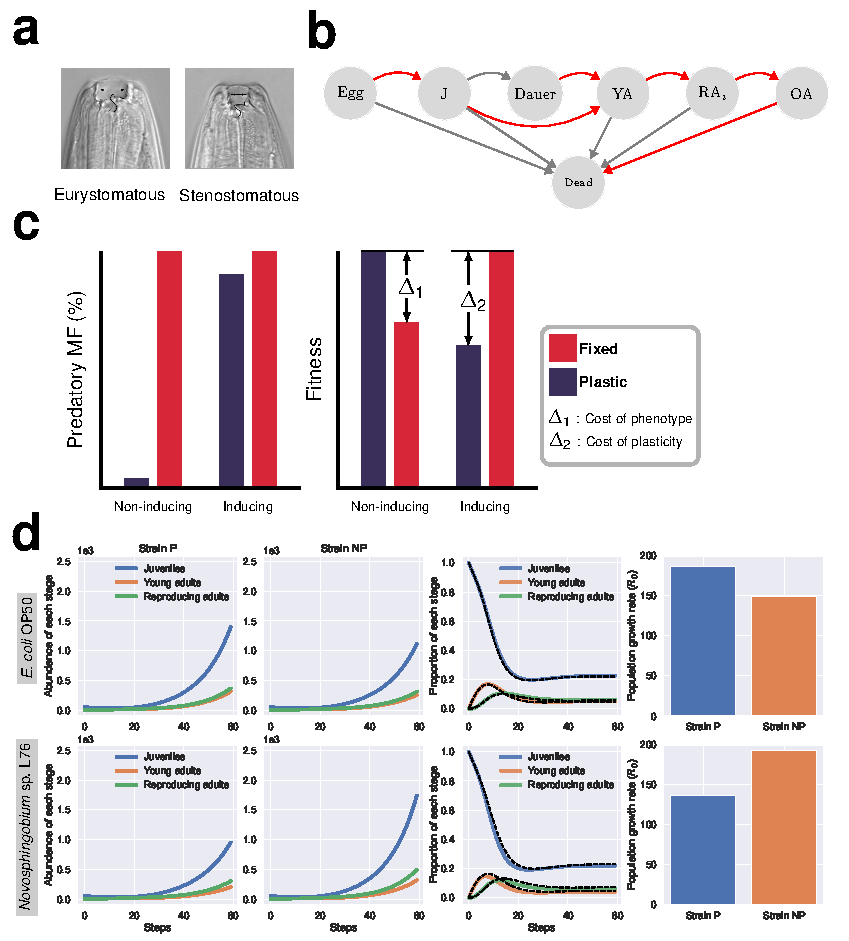
\includegraphics[width=140mm]{figures/figure1.jpg}
\caption{\textbf{Phenotypic plasticity and associated costs in \ppac{}.} \footnotesize (a) The nematode \ppac{} expresses two alternative mouth forms, the predatory (eurystomatous) and the non-predatory (stenostomatous) from, in response to a variety of external stimuli. The fate of the mouth form is determined during post-embryonic development. (b) The life cycle of the worm can be depicted as a Markov chain, where each state corresponds to a developmental stage. The transition rates between different stages in our model are a function of resource availability. The transitions depicted as solid gray lines only happen in the absence of resource. (c) The cost of plasticity and the cost of phenotype in our model can be illustrated in a hypothetical scenario: The plastic strain  switches from the non-predatory mouth form to the predatory mouth form when grown on the inducing diet, but this plastic response to this diet is accompanied by a reduction in fitness, $\Delta_2$, which is the cost of plasticity. The fixed strain expresses the predatory mouth form in both environments, but its fixed phenotype is adapted to the inducing environment, resulting in a cost of (fixed) phenotype in the non-inducing environment ($\Delta_1$). It is evident that costs of phenotype and plasticity are, by definition, exclusively meaningful in comparative studies in environments, which can be described as adaptive and non-adaptive with regards to a given trait. (d) In isolation and in the abundance of resources, our model depicts the population dynamics of the plastic and the non-plastic strains based on the laboratory measurements of fecundity on the two alternative diets. The dashed black lines represent the proportion of each stage for the plastic strain. The simulations started with $50$ juveniles. Abbreviations: J, juvenile; YA, young adult; $\mathrm{RA}_i$, reproducing adult of day $i$; OA, old adult; P, plastic; NP, non-plastic.}
\label{fig:fig1}
\end{flushright}
\end{adjustwidth}
\end{figure}

\begin{figure}
\begin{adjustwidth}{-2in}{0in}
    \begin{flushright}
\includegraphics[width=140mm]{figures/figure2.jpg}
\caption{\textbf{Cost of plasticity in well-mixed versus spatially-structured populations.} \footnotesize (a) The expected outcome of competition between the non-plastic (solid lines) and the plastic strains (dashed black lines) in a population with limited resource. In the absence of predation, the plastic strain would out-compete the non-plastic strains on \ecoli{} given its higher per-generation growth rate. If predation is included, the non-plastic strain is always eliminated by the plastic strain, regardless of the bacterial diet. (b) The meta-population in our model consists of $m \times m$ subpopulations ($S_{1,1}$ to $S_{m, m}$), on a lattice. The dauer larvae can move between connected subpopulations. (c) The movement of dauer larvae in our model is simulated as a simple diffusion, where time $\tau_2$ dauers move according to their diffusion rate and the concentration of dauer larvae at $\tau_1$ in neighboring subpopulations. (d) In each simulation of our metapopulation model, juveniles of the plastic strains are added to $S_{1,1}$ and $S_{m,m}$;  $S_{1,m}$ and $S_{m,1}$ are seeded with juveniles of the non-plastic strain (initial number of juveniles in each subpopulation $=50$). On \ecoli{} the abundance of reproducing adults (RA) of the plastic strain exceeds that of the non-plastic strain and dauer larvae of the plastic strain dominates the metapopulation, whereas on \novo{}, the non-plastic strain wins. For this and the subsequent figures, predation rate $\alpha=0.001$, consumption rate $\rho=0.01$, diffusion rate $r=0.01$, initial resource per subpopulation $R_0 = 1000$, and dimension of the lattice $m=10$.}
\label{fig:fig2}
\end{flushright}
\end{adjustwidth}
\end{figure}

\begin{figure}
\begin{adjustwidth}{-2in}{0in}
    \begin{flushright}
\includegraphics[width=140mm]{figures/figure3.jpg}
\caption{\textbf{The effect of initial resource heterogeneity on the competition between the plastic and the non-plastic strains.} (a) The metapopulation was divided into quadrants and each quadrant was assigned an alternative resource, such that subpopulations seeded with plastic juveniles ($S_{1,1}$ and $S_{m,m}$) are within \ecoli{} quadrants and subpopulations seeded with non-plastic juveniles ($S_{1,m}$ and $S_{m,1}$) within \novo{} quadrants. In this pattern, the non-plastic strain dominates. (b) If we use the alternative pattern, one where subpopulations seeded with plastic juveniles ($S_{1,1}$ and $S_{m,m}$) are within \novo{} quadrants, the result of the competition is drastically altered. (c) Random starting distribution of resource can result in scenarios where the plastic strain dominates the metapopulation.}
\label{fig:fig3}
\end{flushright}
\end{adjustwidth}
\end{figure}

\begin{figure}
\begin{adjustwidth}{-2in}{0in}
    \begin{flushright}
\includegraphics[width=120mm]{figures/figure4.jpg}
\caption{\textbf{The effect of temporal heterogeneity with regards to diet on the competition between the plastic and the non-plastic strains.} (a) We injected resources of a given type (\ecoli{} or \novo{}) each $100$ steps (henceforth referred to as cycles) to the metapopulation. Upon the injection of food, dauer larvae develop into young adults. If we alternate between \ecoli{} and \novo{} each cycle, the number of reproducing adult of both strains remain relatively comparabale, but the non-plastic strain eventually wins out. (b) If we alternate between \ecoli{} and \novo{} every two cycles, the plastic strain competitvly excludes the non-plastic strains. (c) This pattern holds even after we increase the number of \novo{}  cycles. (d) Random alternation between the two bacterial diets can produce a variety of outcomes, including scenarios where both strains transiently coexist in the metapopulation.}
\label{fig:fig4}
\end{flushright}
\end{adjustwidth}
\end{figure}


\nolinenumbers

\clearpage

%This is where your bibliography is generated. Make sure that your .bib file is actually called library.bib
\bibliography{library}
%This defines the bibliographies style. Search online for a list of available styles.
\bibliographystyle{abbrv}

\clearpage
\newpage

\section*{Supplementary figures}

\setcounter{figure}{0}    

%\renewcommand{\figurename}{Figure}
\renewcommand{\thefigure}{S\arabic{figure}}

\begin{figure}
\begin{adjustwidth}{-2in}{0in}
    \begin{flushright}
\includegraphics[width=130mm]{figures/figureS1.jpg}
\caption{\textbf{The effect of the diets and low resource on the transition and survival probabilities in the model.} \novo{} deferentially affects the transition between YA and day-one reproducing adult (RA$_1$) in the plastic (P) and the non-plastic strains (NP), reflecting our experimental observations. The transition probabilities are chosen such that the occupancy time in the Markov chain, calculated using the fundamental matrix ($\mathbf{N} = (\mathbf{I} - \mathbf{U})^{-1}$), approximately corresponds to the life-cycle of \emph{P.pacificus} in hours, e.g., transition probability $0.0415$ results in an occupancy time of $\approx 24$ steps. The low resource condition is satisfied when $\mathcal{R}_t \leq \mathcal{R}_\mathrm{min}$, where $\mathcal{R}_\mathrm{min} = 100$.}
\label{fig:figs1}
\end{flushright}
\end{adjustwidth}
\end{figure}

\begin{figure}
\begin{adjustwidth}{-2in}{0in}
    \begin{flushright}
\includegraphics[width=140mm]{figures/figureS2.jpg}
\caption{\textbf{Random initial distribution of resource does not always favor the plastic strain.} The population dynamics of the plastic and the non-plastic strains on four metapopulations with random initial resource distributions are shown. In each case,  \ecoli{} or \novo{} was randomly assigned to each subpopulation.}
\label{fig:figs2}
\end{flushright}
\end{adjustwidth}
\end{figure}


\begin{figure}
\begin{adjustwidth}{-2in}{0in}
    \begin{flushright}
\includegraphics[width=120mm]{figures/figureS3.jpg}
\caption{\textbf{Random alteration between two diets results in alternative competitive outcomes.} The population dynamics of the plastic and the non-plastic strains with random alteration patterns.}
\label{fig:figs3}
\end{flushright}
\end{adjustwidth}
\end{figure}

\begin{figure}
\begin{adjustwidth}{-2in}{0in}
    \begin{flushright}
\includegraphics[width=180mm]{figures/figureS4.jpg}
\caption{\textbf{The dynamics of the plastic and the non-plastic strain on a toroidal metapopulation.} To ensure that the patterns observed on the metapopulation is not an artifact of the dispersion pattern, we repeated the simulation on $16\times16$ lattice with the periodic boundary condition, i.e., a torus-shaped metapopulation. The white squares represent the subpopulations that were seeded with the plastic strain, $S_{4,4}$ and $S_{13,13}$, and the non-plastic strain, $S_{4,13}$ and $S_{13,4}$. The results on torus-shaped metapopulations are consistent with our previous results.}
\label{fig:figs4}
\end{flushright}
\end{adjustwidth}
\end{figure}



\end{document}

